\documentclass[10pt]{article}
% Packages
\usepackage{makecell} % For thicker lines
\usepackage{setspace}  % Controls line spacing
\usepackage{hhline}   % For double horizontal lines
\usepackage{colortbl}  % Add colour to LaTeX tables
\usepackage[T1]{fontenc}  % Choice of font encodings
\usepackage{tgtermes}  % Loads the TeX Gyre Termes font
\usepackage{siunitx}  % A comprehensive (SI) units package
\usepackage{tabularx, booktabs} % For advanced table layout
\usepackage{url}  % Verbatim with URL-sensitive line breaks
\usepackage{authblk}  % For author and affiliation management
\usepackage{natbib}  % A package for bibliographies and citations
\usepackage{graphicx}  % Enhances LaTeX's built-in graphics features
\usepackage{listings}  % Typeset programming code within the document
\usepackage{amssymb}  % Mathematical symbols
\usepackage[nottoc]{tocbibind}  % Adds entries to the table of contents
\usepackage{xcolor}  % Provides easy driver-independent access to colors
\usepackage{microtype}  % Improves the spacing between words and letters
\usepackage{enumitem}  % Control layout of itemize, enumerate, description
\usepackage{tocloft}  % Controls the typographic design of table of contents, etc.
\usepackage[breaklinks,linktocpage]{hyperref}  % Creates hyperlinks in your document
\usepackage[font=small,skip=7pt,labelfont=bf]{caption}  % Customising captions in floating envs

% Adjust the page margins in the bibliography
\let\oldthebibliography=\thebibliography
\let\endoldthebibliography=\endthebibliography
\renewenvironment{thebibliography}[1]{%
  \begin{oldthebibliography}{#1}%
    \raggedright%
    }{%
  \end{oldthebibliography}%
}

\setlength\bibindent{0pt}

% Optional options
% \usepackage{background} % Creates a DRAFT background image on all pages
% \backgroundsetup{contents=Preprint, opacity=0.25, color=gray} % Adds a watermark to the document
% This command changes the line spacing to double.
% ? Needed for reviews/drafts
% \doublespacing

% Custom colours
\definecolor{codegreen}{rgb}{0,0.5,0}
\definecolor{codegray}{rgb}{0.4,0.4,0.4}
\definecolor{codepurple}{rgb}{0.58,0,0.82}
\definecolor{backcolour}{rgb}{0.96,0.96,0.96}
\definecolor{lightgray}{gray}{0.8}

\lstdefinelanguage{JavaScript}{
  keywords={break, case, catch, continue, debugger, default, delete, do, else, finally, for, function, if, in, instanceof, new, return, switch, this, throw, try, typeof, var, void, while, with},
  morecomment=[l]{//},
  morecomment=[s]{/*}{*/},
  morestring=[b]',
  morestring=[b]",
  sensitive=true
}

% Listing styles
\lstdefinestyle{mystyle}{
  frame=tb,
  tabsize=2,
  captionpos=b,
  numbers=left,
  framerule=0pt,
  numbersep=5pt,
  showtabs=false,
  breaklines=true,
  keepspaces=true,
  showspaces=false,
  framextopmargin=6pt,
  framexbottommargin=6pt,
  showstringspaces=false,
  breakatwhitespace=false,
  keywordstyle=\color{purple},
  commentstyle=\color{codegreen},
  stringstyle=\color{codepurple},
  numberstyle=\tiny\color{codegray},
  basicstyle=\ttfamily\footnotesize,
  backgroundcolor=\color{backcolour}}
\lstset{style=mystyle}

% ! Custom template commands
% Add a vertical space after section numbers in ToC
\renewcommand\cftsecafterpnum{\vskip8pt}
% Changes the title of the list of listings
\renewcommand{\lstlistlistingname}{List of \lstlistingname s}
% Changes the title of the bibliography
\renewcommand{\bibname}{References}
% Changes the title of the table of contents
\renewcommand{\contentsname}{Table of Contents}
% Changes the leader between section and page numbers in ToC
\renewcommand{\cftsecleader}{\cftdotfill{\cftdotsep}}
\newcommand{\floatcaption}[2]{\caption[#1.]{#1~#2.}}

% Custom template settings
\captionsetup{justification=centering}  % All captions will be centered
\hypersetup{
  colorlinks = true,
  urlcolor = blue,
  linkcolor = blue,
  citecolor = blue,
  breaklinks = true
}
\PassOptionsToPackage{hyphens}{url}
\urlstyle{same}
\def\Urlmuskip{0mu plus 1mu}
\def\UrlBreaks{\do\/\do-}
\def\UrlBigBreaks{\do\/\do-\do:\do.}
\setlist[itemize]{noitemsep, topsep=0pt, partopsep=0pt}



\begin{document}
\pagenumbering{roman}
\counterwithin{lstlisting}{section}
\counterwithin{figure}{section}
\counterwithin{table}{section}
\setlength{\footskip}{65pt}

% ! ===========================
% ! # MARK: Title, author, etc.
% ! ===========================

\title{\textbf{Lab-Grown Human Brain \\ Embodied in a Virtual World}}
\author[1]{Daniel Burger}
\affil[1]{\textbf{FinalSpark Sàrl}}
\affil[ ]{\href{mailto:public@danielburger.online}{public@danielburger.online}}
\date{\textit{October 18, 2024}}
\maketitle
\thispagestyle{empty}

\begin{sloppypar}

  \begin{figure}[ht]
    \centering
    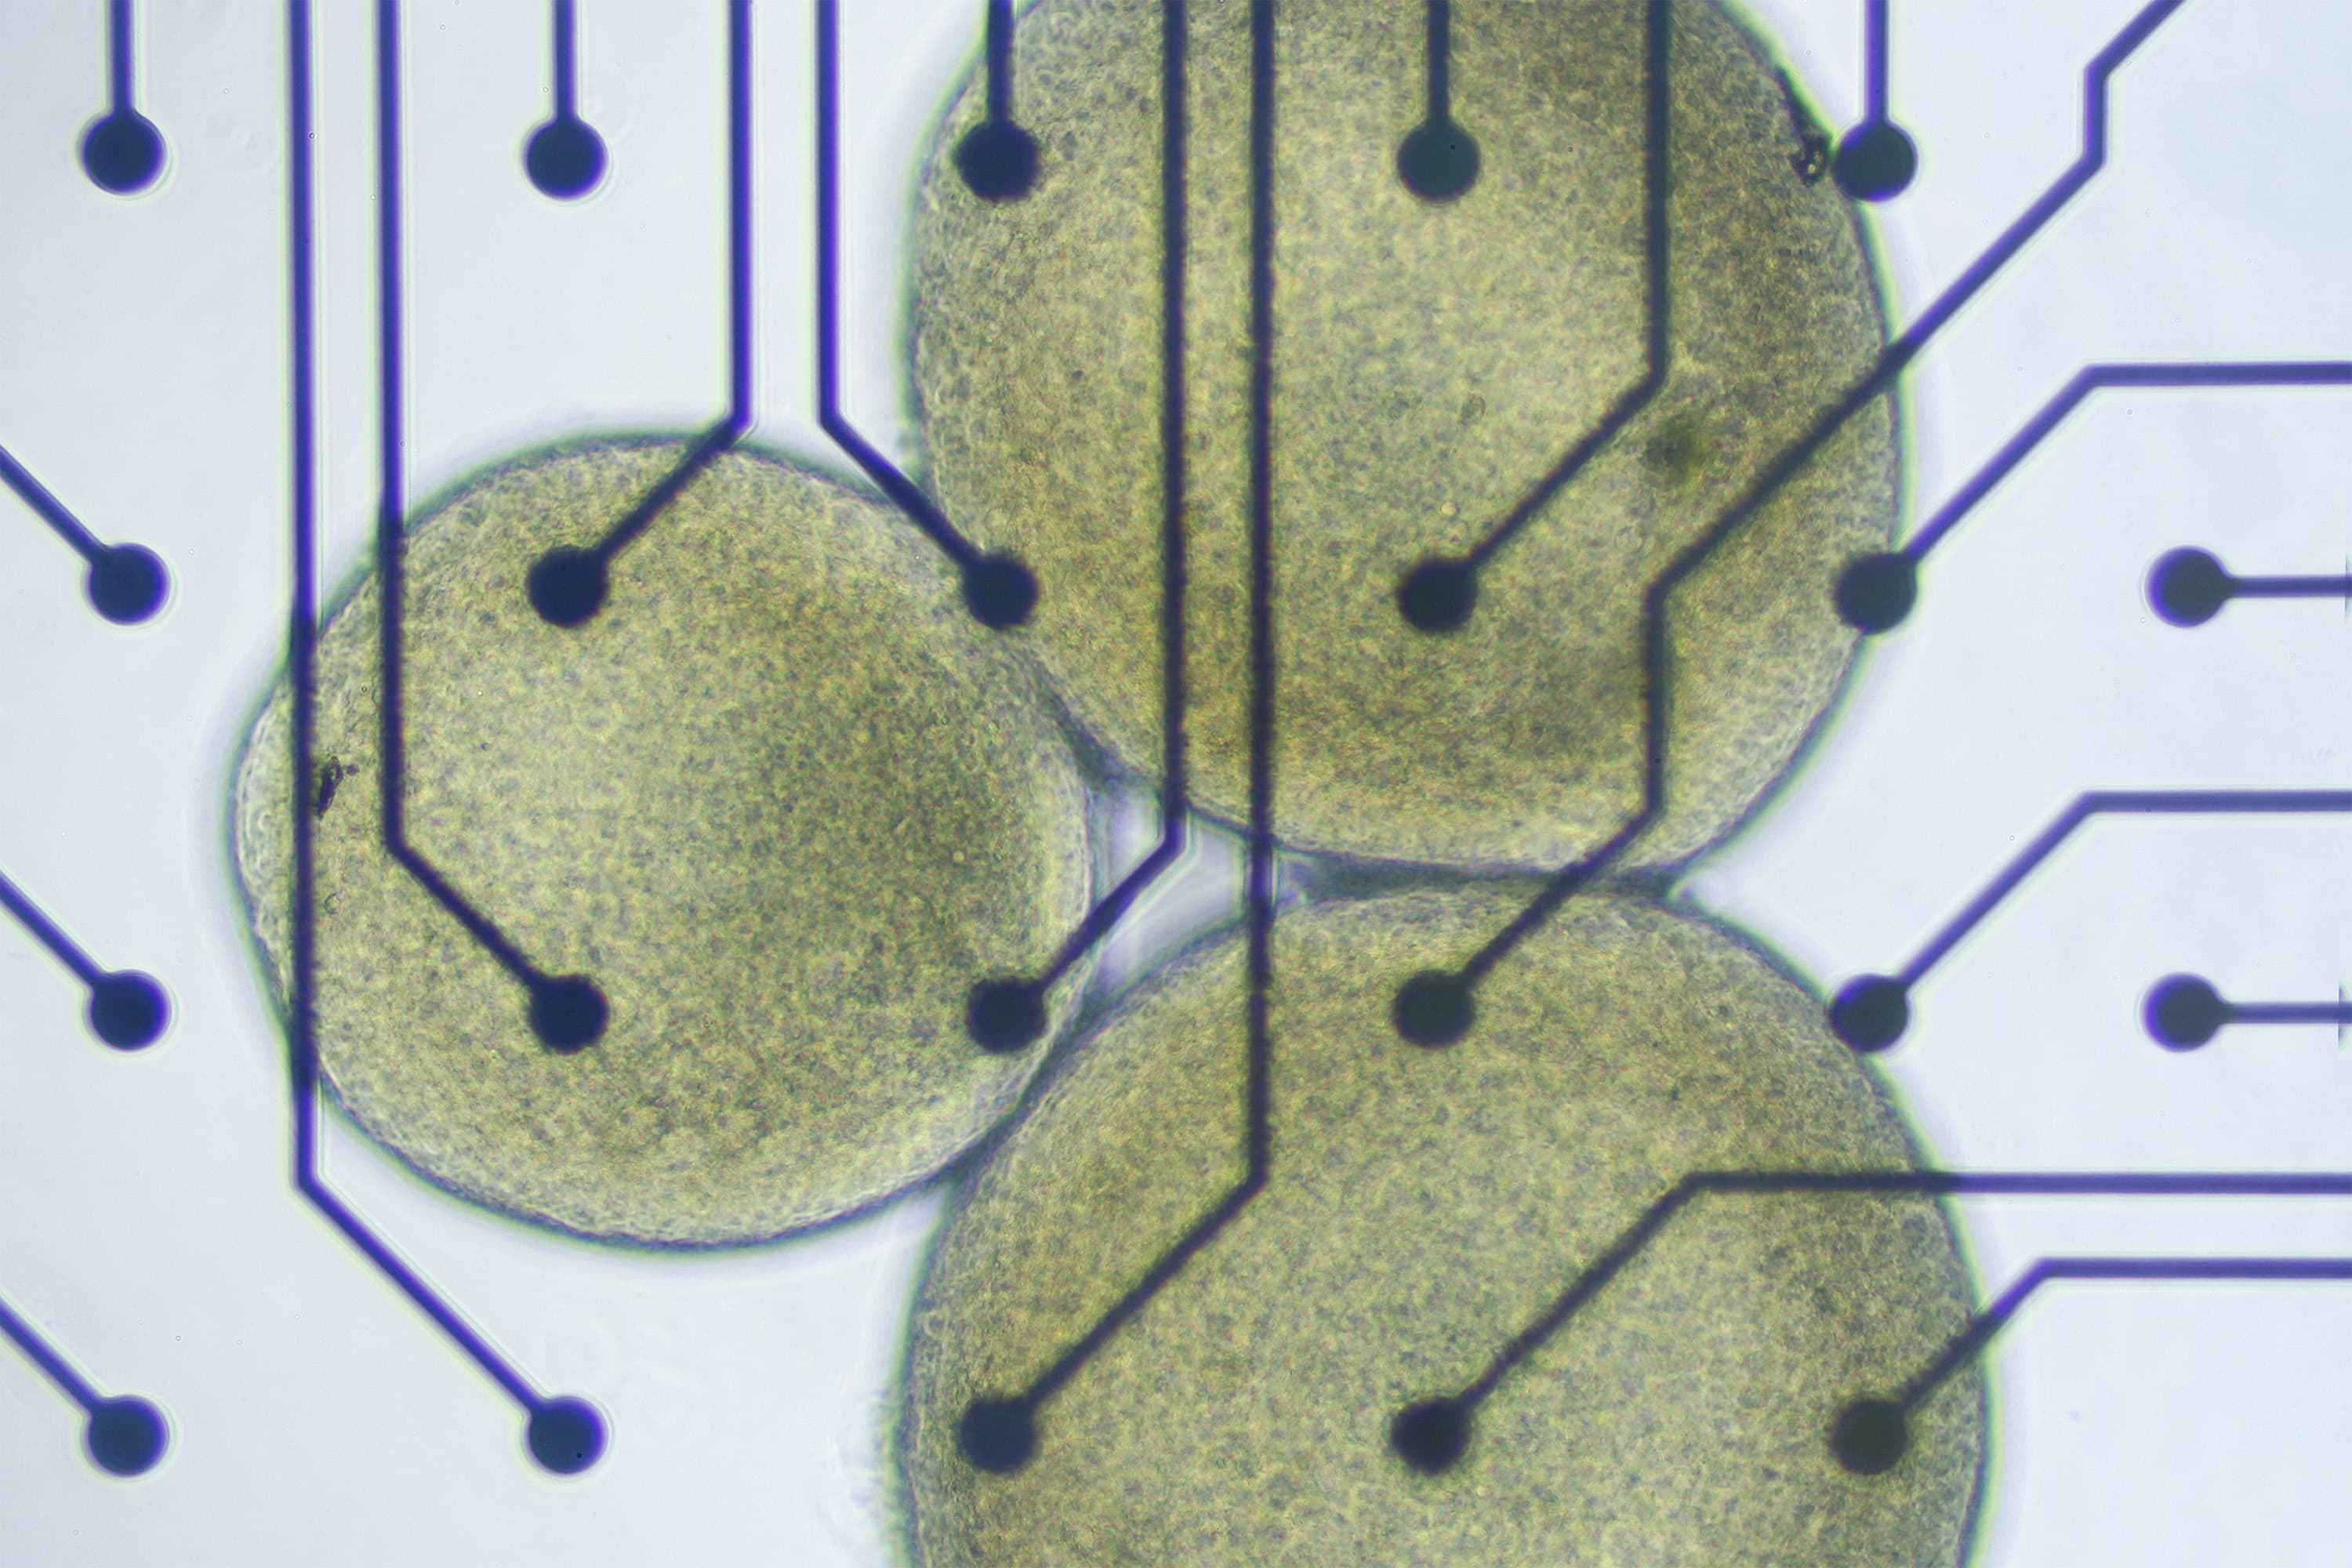
\includegraphics[width=\textwidth]{figures/cover.jpg}
    \label{fig:cover}
  \end{figure}

  \begin{abstract}
    Our team put a human mini-brain into virtual reality and let people interact with it over the internet. It's the first time anyone has done this, and we'd like to share the behind-the-scenes with you.
    % TODO Add more content to abstract.
  \end{abstract}

  \pagebreak
  \pagenumbering{Roman}
  \tableofcontents
  \pagebreak
  \listoffigures
  \pagebreak
  \listoftables
  \pagebreak
  \addcontentsline{toc}{section}{\lstlistlistingname}
  \lstlistoflistings
  \pagebreak
  \pagenumbering{arabic}

  % ! ========================
  % ! # MARK: Document content
  % ! ========================

  \section{Introduction}
  \label{sec:introduction}

  Earlier this year, I had the opportunity to work on a project with FinalSpark, a Swiss startup developing the world's first wetware cloud platform. We created the Neuroplatform, a system that enables researchers and developers to interact remotely with human brain organoids. Our platform essentially allows 'running software' on biological neural networks (BNNs), with the ultimate goal of achieving and deploying synthetic biological intelligence.

  \begin{figure}[ht]
    \centering
    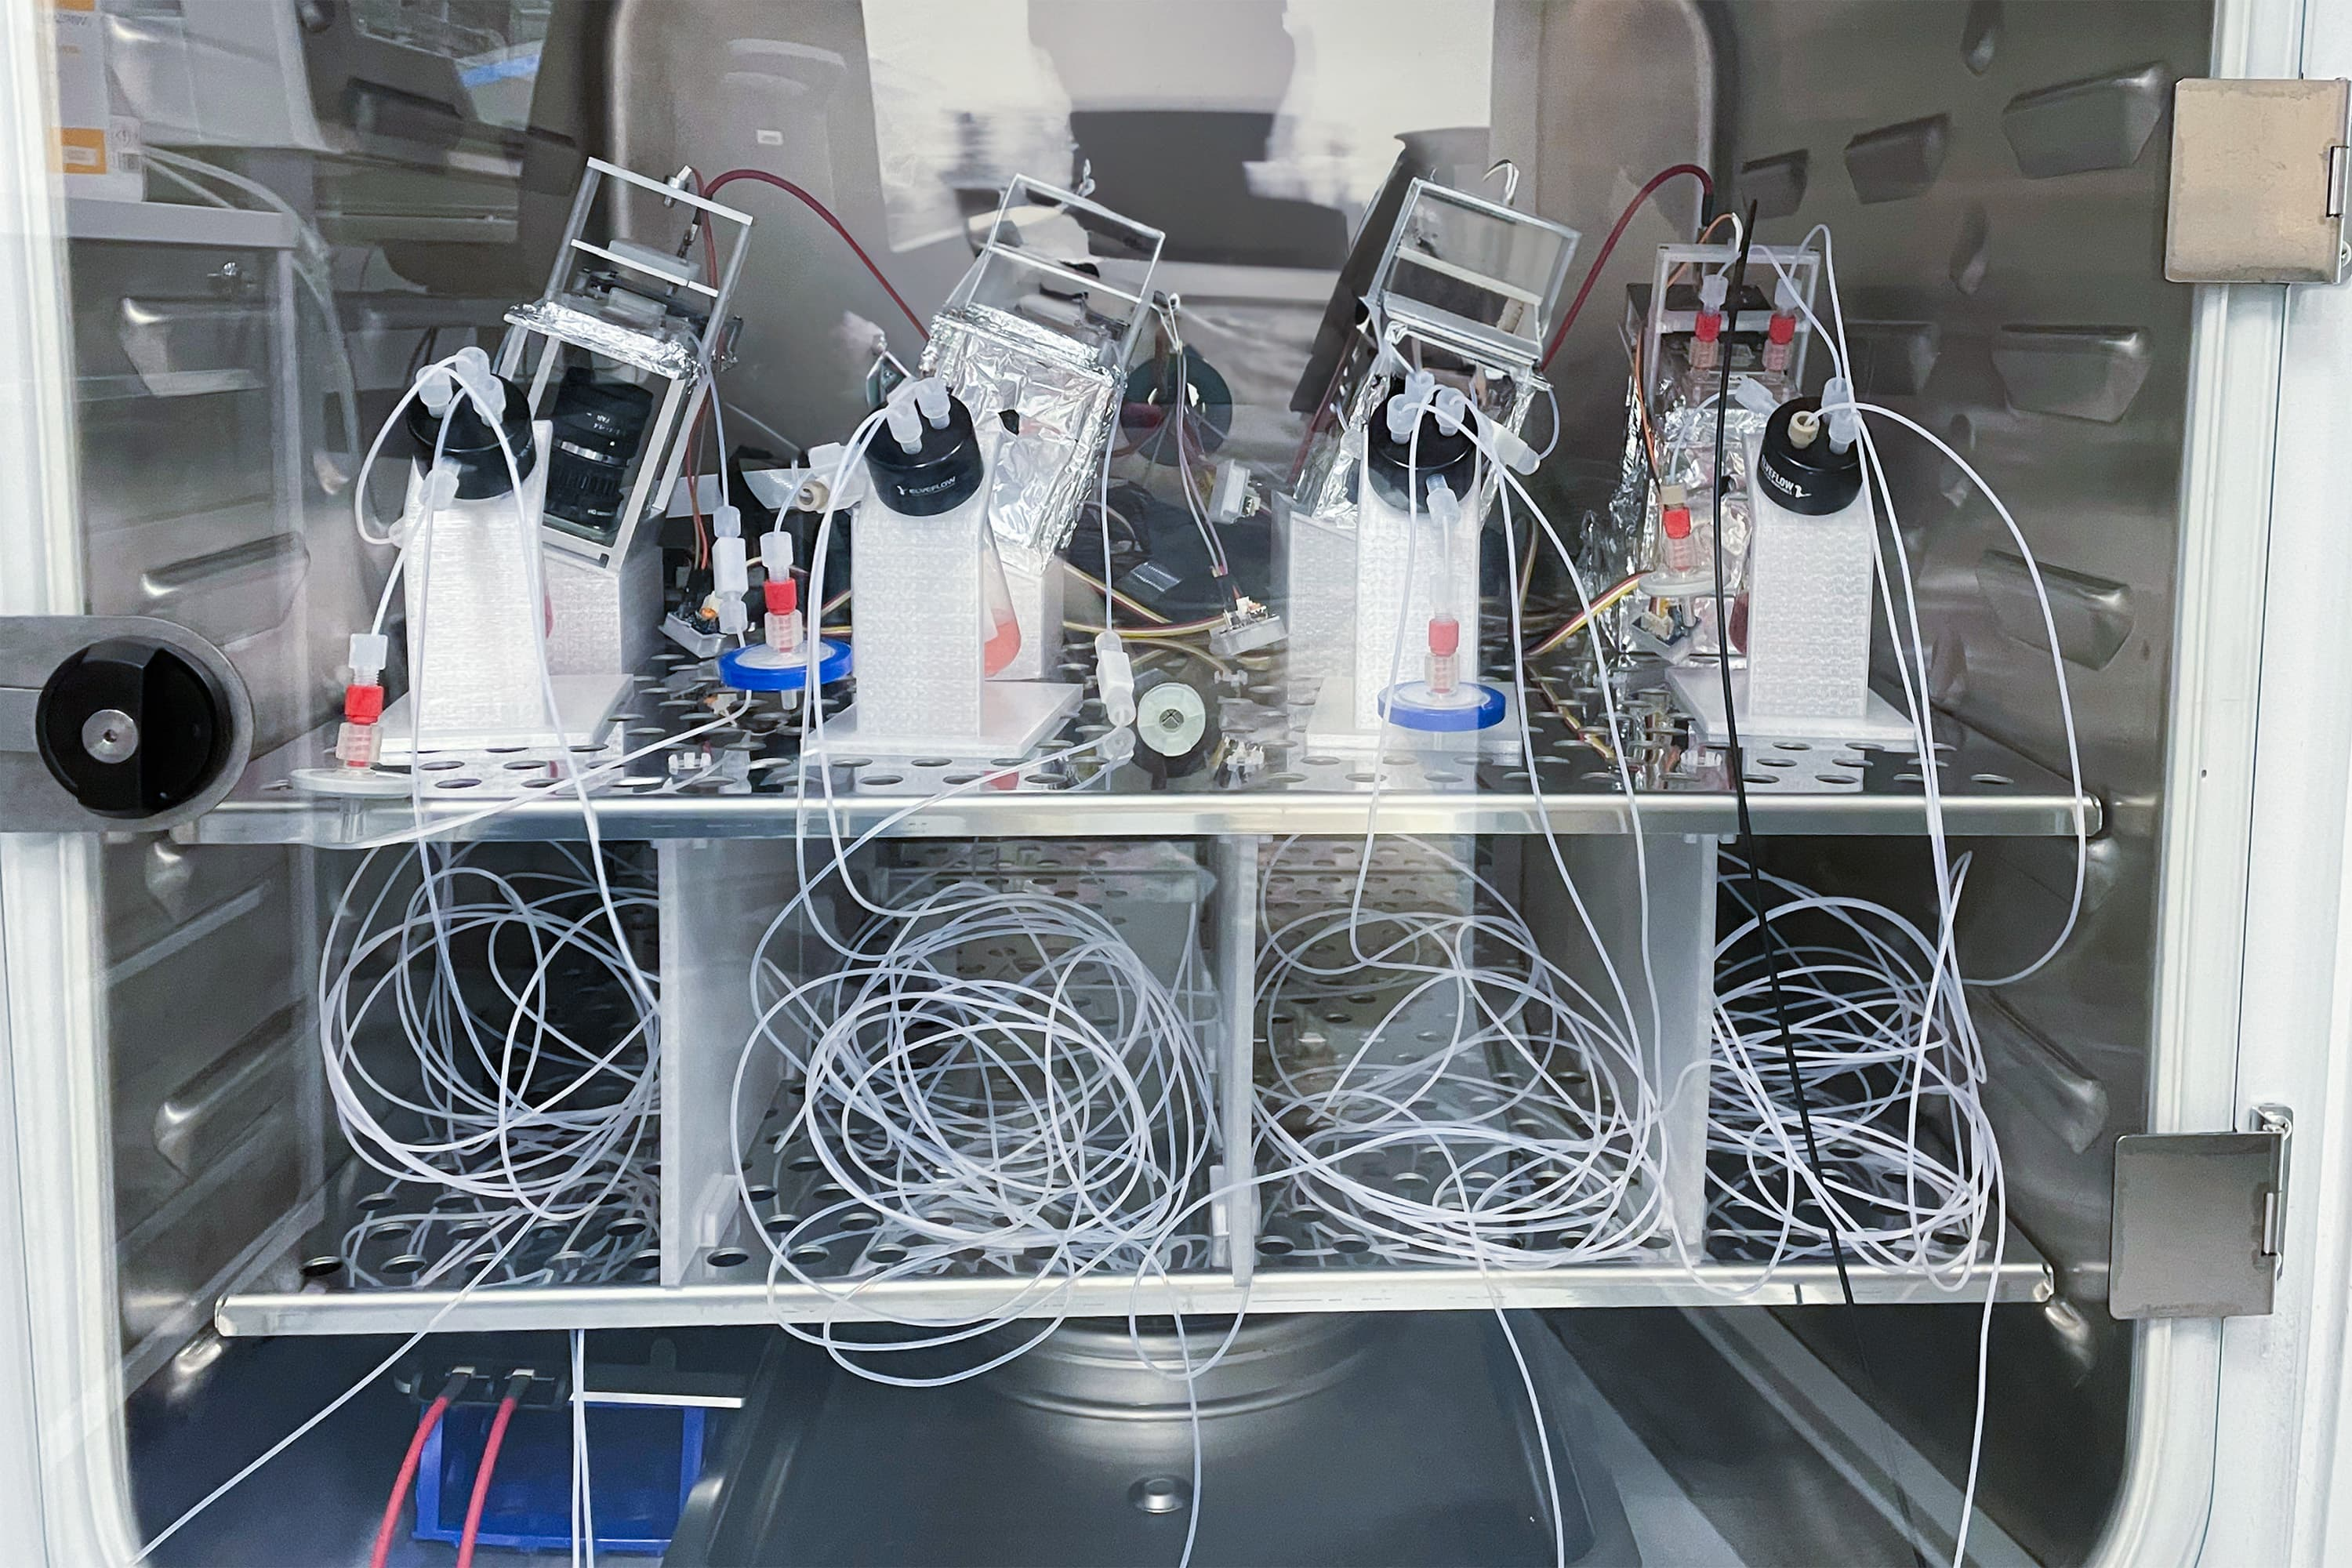
\includegraphics[width=\textwidth]{figures/incubator.jpg}
    \caption[Brain organoid incubator at FinalSpark lab]{A look into the incubator inside the lab at FinalSpark, where our brain organoids are connected to various systems to keep them alive and ultimately connected to the internet.}
    \label{fig:incubator}
  \end{figure}

  The potential benefits of BNNs over traditional silicon-based artificial neural networks (ANNs) are numerous, though they are mainly theoretical today. Nonetheless, the advantages include significantly lower energy consumption (the human brain operates on only about 20 watts \citep{balasubramanian_brain_2021}), truly higher cognitive and adaptive behaviour such as creativity, true zero-shot learning capabilities, superior pattern recognition and generalisation, better handling of ambiguity and noise, and the potential for self-repair and neuroplasticity.

  The Neuroplatform currently hosts 16 active brain organoids, with the potential to rapidly deploy many more from our extensive stock of neural progenitors stored in liquid nitrogen. These mini-brains, derived from induced pluripotent stem cells (iPSCs), are maintained in incubators at 37°C (shown in \autoref{fig:incubator}), closely mimicking the intracranial conditions of the human body. Each organoid, comprising approximately 10,000 neurons, interfaces with a multi-electrode array (MEA) for bidirectional electrical communication. The platform also incorporates a sophisticated microfluidic system and an ultraviolet light-controlled uncaging mechanism, enabling precise delivery of nutrient media, neurotransmitters, and neuromodulators like dopamine and serotonin, thus closely replicating the functional environment of the human brain.

  \begin{quote}
    \itshape
    \textbf{What is a Brain Organoid?}
    A brain organoid is a three-dimensional cellular model of the human brain grown in a laboratory from stem cells. These miniature "mini-brains" are typically the size of a pea or smaller and contain various types of brain cells organised in a structure that mimics aspects of a developing human brain. While they don't have the full complexity of an adult human brain, brain organoids can develop basic neural circuits and exhibit spontaneous electrical activity.

    Researchers usually use brain organoids to study human brain development and neurological disorders and, more recently, as is the case with FinalSpark, as biological/wetware computing components.
  \end{quote}

  As a research and development engineer in our small team, I was crucial in developing the Neuroplatform’s foundation, application programming interface (API), and software development kit. Our system empowers researchers to conduct complex experiments, including reinforcement learning, reservoir computing, and synaptic connectivity studies, to name a few. Our work builds upon the foundations laid by pioneers in the field, such as Steve M. Potter (who is actually an advisor to FinalSpark) and Wolfram Schultz. Beyond the fundamental neurobiology, organoid cultivation, and hardware development, our research explores the concept of “world-model-dependent intelligence”. This involves embedding brain organoids in virtual environments to study their ability to infer patterns from data, act upon them, and, most notably, learn from these interactions—a holy grail in organoid intelligence research.

  \begin{quote}
    \itshape
    \textbf{Who started working on organoid intelligence?}
    The field now known as organoid intelligence (OI) has its roots in early work on cultured neuronal networks. In the late 1990s and early 2000s, Dr. William L. Ditto at the Georgia Institute of Technology was among the first to explore the computational capabilities of living neuronal networks.

    Building on this foundation, in the early 2000s, Dr. Steve M. Potter, also at Georgia Tech, pioneered research on “hybrots” (hybrid robots) and embodied cultured networks. Then, a significant leap came in 2013 when Dr. Madeline Lancaster and her lab developed the first protocol for creating cerebral organoids, providing a powerful new tool for researchers.

    The field gained additional momentum with Dr. Kagan’s 2022 study showing that neural cultures could learn to play Pong. In 2023, Dr. Thomas Hartung and his team at Johns Hopkins University coined the term “organoid intelligence”, synthesising previous work and outlining future directions.
  \end{quote}

  To showcase the Neuroplatform’s capabilities, we developed an interactive demo that allows users to indirectly “control” a brain organoid in real-time. Initially conceived by FinalSpark’s CEOs in early 2023, the concept evolved into a virtual butterfly whose flight path can be steered by a user-controlled “target” (e.g., food or light). When the butterfly “sees” the target, it flies towards it; otherwise, it meanders randomly, mimicking natural butterfly behaviour. While the idea seems simple, its implementation proved challenging in terms of neural interfacing, software engineering, and user experience design. To ensure widespread accessibility, we created the demo as a web application and web service, eliminating the need for software downloads or direct connections to the Neuroplatform’s internal network. But before going into the technical nitty-gritty of the demo and its interface with the brain organoids—aspects that I anticipate will interest most readers—I’d like to direct your attention to our recent peer-reviewed publication in Frontiers.

  Our paper provides a comprehensive overview of the Neuroplatform’s technical and scientific foundations, offering valuable context beyond the butterfly demo. It marks our official introduction of the Neuroplatform to the scientific community and is an excellent resource for those seeking a deeper understanding of the underlying electronics and neurobiology.

  % ! ========================
  % ! # MARK: References, etc.
  % ! ========================

  \pagebreak
  \bibliographystyle{../../templates/custom-apa}
  \bibliography{references/bibliography}
  \nocite{*}

\end{sloppypar}
\end{document}
